\section{Desarrollo}

\subsection{Calibración}

El primer paso para comenzar el algoritmo de fotogrametría estéreo es realizar
la calibración del sistema. Cada imágen tiene una fuente de iluminación. Cada
fuente tiene una dirección en la que apunta su luz. El objetivo del paso de
calibración es poder calcular la dirección de cada fuene de iluminación.

Cada objeto tiene 12 imágenes del mismo con fuentes de iluminación con
distintas direcciones. Estas 12 fuentes de iluminación son distintas entre sí,
pero se repiten para todos los objetos. Esto hace posible que si pudiesen
calcularse las direcciones de las 12 fuentes para un objeto en particular,
entonces podrían reutilizarse para el resto de los objetos.

En este caso pueden calcularse las direcciones de las fuentes de iluminación
de uno de los objetos: la esfera. Lo que permite que esto sea posible es el
hecho de conocer con exactitud la profundidad del objeto. Al saber que el
objeto es una esfera, puede conocerse con exactitud la posición de cada
punto, sabiendo el centro y el radio de la misma siguiendo la siguiente
ecuación:

\begin{center}
$(x - x_0)^2 + (y - y_0)^2 + (z - z_0)^2 = r^2$
\end{center}

donde $z_0 = 0$ ya que suponemos que está centrada respecto del eje z.
Gracias a esto, puede calcularse el vector normal a cada punto de la esfera

\begin{center}
$n = (x - x_0, y - y0, z)$
\end{center}

Sabemos, dada la naturaleza de la esfera, que el punto de mayor intensidad
lumínica será el más cercano a la fuente de iluminación, por lo que la normal
de dicho punto apuntará en dirección a la fuente. El vector opuesto a esta
normal tiene la dirección de la fuente.

Si se ejecuta este procedimiento para las 12 imágenes de la esfera, entonces
el resultado será conocer la dirección de las 12 fuentes de iluminación. Esto
permite, en los pasos siguientes del algoritmo de fotogrametría estéreo,
poder calcular la normal para cada punto, basándose en que la fuente de
iluminacion $s_i$ con $1 \leq i \leq 12$ es la misma para la imágen $i$ de
cada objeto.

\subsection{Reconstrucción del modelo 3D de los objetos digitalizados}

Una vez completada la calibración, ya se cuenta con las direcciones de
iluminación de cada caso, las cuales junto con la secuencia de imágenes de un
objeto nos proporcionarán la información necesaria para poder calcular todos
los puntos $(x,y,z)$ del modelo digitalizado y las normales de cada uno.

Puede dividirse en:

\begin{enumerate}
\item Construcción del campo normal
\item Estimación de la profundidad
\end{enumerate}

\subsubsection{Contrucción del campo normal}

En este paso se desea obtener la normal de cada punto del objeto. Para ello
se recurre a la ecuación 5 del enunciado de este trabajo práctico, que
vincula una matriz formada por 3 direcciones de fuentes de iluminación con el
vector $m$ y las intensidades del píxel en cada imágen. Esta matriz tiene 3
direcciones porque es la cantidad mínima de imágenes cuya fuente de
iluminación difiera entre sí necesaria para inferir la orientación de la
superficie.

La matriz de direcciones contiene la dirección de cada fuente de iluminación
dispuesta como fila. Una vez resuelto el sistema de ecuaciones se podrá conocer $m$ y asi mediante la siguiente ecuacion $||m|| = |I_0\rho| ||n||$, conocer el valor absoluto de $I_0\rho$. Esto permite conocer $n$ ya que tiene la misma dirección que $m$ con la diferencia de que $n$ está normalizado por ser la norma. Por lo que nos queda que $n = \frac{m}{||m||}$.

\subsubsection{Estimacion de la profundidad}

El siguiente paso es calcular la profundidad de cada pixel de la imagen. Para ello se recurre a las ecuaciones 11 y 12 del enunciado en donde se vincula a la normal de cada pixel con su profundidad. Estas ecuaciones nos permiten formar un sistema de ecuaciones como el de la ecuación 13.

Es necesario notar que $M$, la matriz de este sistema, es una matriz esparsa. La manera en la que la está dispuesta la información es la siguiente:

$M$ tiene dimensión $2n \times n$. Esto es porque necesitamos representar 2 ecuaciones por cada pixel, por lo que cada columna de $M$ referirá a $1$ pixel de la imagen y cada fila a una ecuación. Dado que cada pixel utiliza en las ecuaciones a los pixels de la derecha y de abajo, cada columna tendrá a lo sumo 4 elementos (dos por sus propias ecuaciones, una vez por el pixel de su izquierda y otra por el de arriba). Para el caso de los pixels de los bordes derechos e inferiores, solamente tendrán 2 elementos, que se dan por los pixeles que estan en la anteúltima columna y anteúltima fila de la imagen correspondientemente. El último pixel, el que se encuentra en la esquina inferior derecha, no tendrá ningún elemento en su respectiva columna.


Nuestra implementación consiste en considerar a esta matriz como un tipo especial de matriz (la esparsa), para la cual no se tiene un arreglo bidimensional como sería el caso habitual sino un vector de hashmap, donde cada elemento del vector representa una columna. Cada hashmap contendrá entonces 4 elementos o menos. Esto permite que al querer multiplicar una columna por otra (como ocurre en el caso de querer calcular $M^tM$) no sea necesario recorrer toda la columna sino únicamente los elementos distintos de 0. Esta optimización es crucial para el desarrollo del algoritmo a nivel temporal. Además, por cuestiones implementativas, se decidió utilizar un diccionario que mapea cada pixel a una columna, para así poder ubicar rápidamente en $z$ (una vez resuelto el sistema) el valor correspondiente a cada pixel.

Luego resta resolver el sistema de la ecuación 15. Para ello aplicamos la factorización de Cholesky, que también resulta optimizada debido a tratarse de una matriz esparsa, ya que para el cálculo de la matriz triangular inferior es necesario recorrer lo calculado en las iteraciones previas, y al utilizar la implementación de matriz esparsa definida anteriormente se logra recorrer la matriz solamente en los elementos distintos de 0.


\subsection{Experimentación}

En este trabajo se realizaron una serie de experimentaciones para poder responder preguntas planteadas en el enunciado. Se explica el detalle de las respuestas obtenidas en las siguientes subsecciones, pero a modo de introducción de esa parte indicamos que no se obtuvieron respuestas para todas las respuestas, pero las pruebas sirvieron para acercarse a una idea de las mismas.

\subsubsection{Análisis cuantitativo}



\subsubsection{Análisis cualitativo}

\paragraph{Luces por calibración VS Luces de la cátedra}

\paragraph{Calibración y repercusiones}

\paragraph{Elección de las luces}
\

A lo largo del desarrollo, se observó que utilizando las mismas luces se obtenian diferentes calidades de modelos 3D para las distintas imágenes. Esto generó dudas de si el algoritmo para la reconstrucción del modelo estaba bien hecho ya que supusimos que la calidad debería ser igual para todas si se usaba siempre las mismas luces, pero al ver que para algunas imagenes funcionaba mejor que para otras, se llegó a esta experimentación.

Para el caso, se tomaron las imágenes del buda y del gato y se procedió a probar distintas combinaciones de luces, todas obtenidas en base a la calibración, las cuales son una por cada imagen de calibración.

En las imágenes siguientes, se pueden observar los modelos (en las primeras dos) obtenidos utilizando las mismas luces (1, 2 y 3), mientras que en las segundas dos se muestran las profundidades del gato y del buda respectivamente.

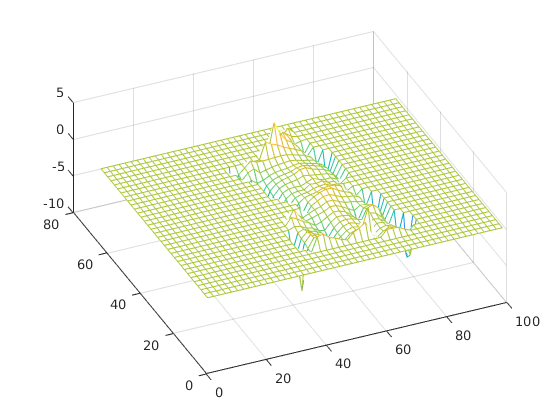
\includegraphics[width=.4\linewidth]{imagenes/gato_small_model_123.png}
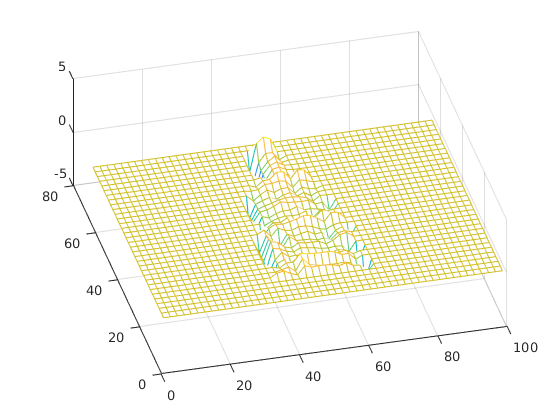
\includegraphics[width=.4\linewidth]{imagenes/buda_small_model_123.png}

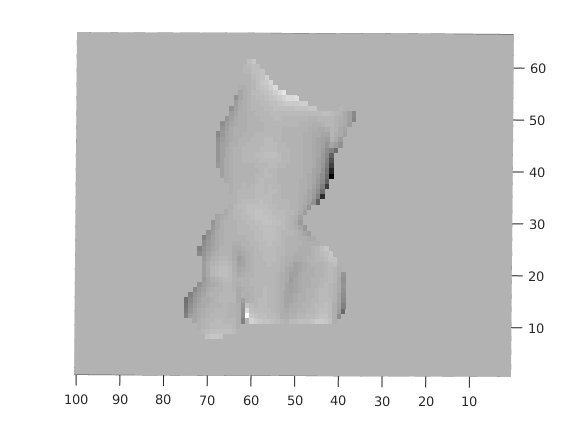
\includegraphics[width=.4\linewidth]{imagenes/gato_small_dephs_123.png}
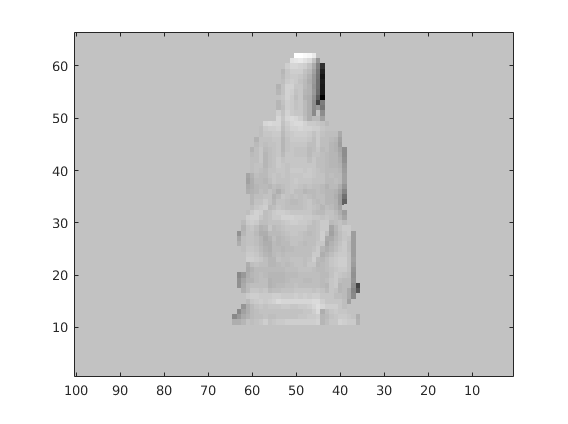
\includegraphics[width=.4\linewidth]{imagenes/buda_small_dephs_123.png}

En esta primera comparación se notó que el modelo y las profundidades del gato tenían una forma mejor detallada que el buda, aunque sólo con esta primera idea no se obtuvo ninguna conclusión, por lo que se continuó con las luces 4, 5 y 6. Sin embargo, al querer utilizar ese conjunto de luces se obtuvieron resultados completamente vacíos. La conclusión a la que se llegó para poder explicar este suceso luego de realizar pruebas fijando una y después dos luces, y cambiando las otras, fue que las luces 3 y 5 son vectores que no son linealmente independientes, ya que dejando fijas esas luces siempre se obtenían modelos vacíos. La razón por la que se concluyó que las luces 3 y 5 no son $L.I.$ fue que al hacer eliminación gausseana, se obtenían filas de $0$s y eso es lo que luego generaría $0$s en las normales estimadas y por lo tanto en todo el modelo.

Después de ese pequeño análisis, se precedió a realizar la generación de modelos 3D con las luces 7, 8 y 9 y los modelos obtenidos fueron los siguientes:

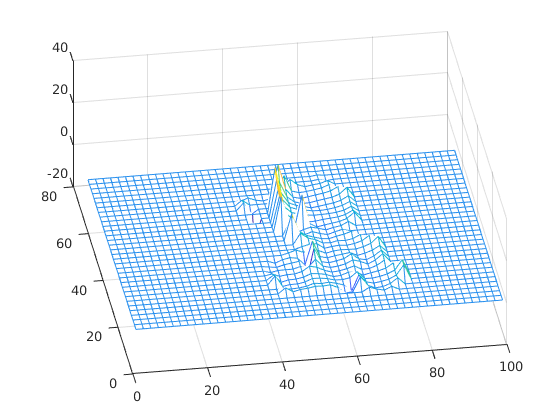
\includegraphics[width=.4\linewidth]{imagenes/gato_small_model_789.png}
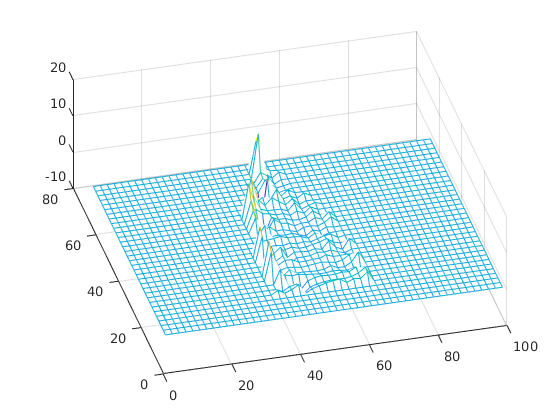
\includegraphics[width=.4\linewidth]{imagenes/buda_small_model_789.png}

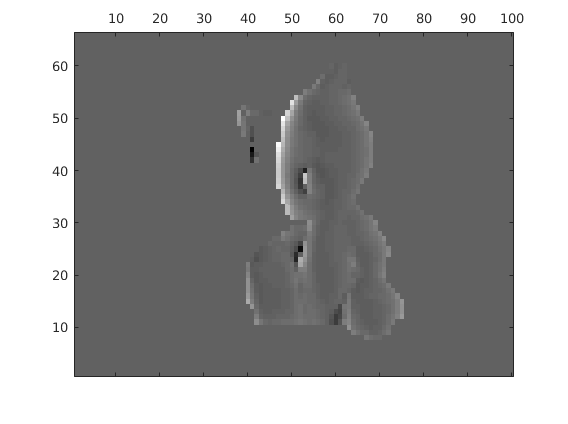
\includegraphics[width=.4\linewidth]{imagenes/gato_small_dephs_789.png}
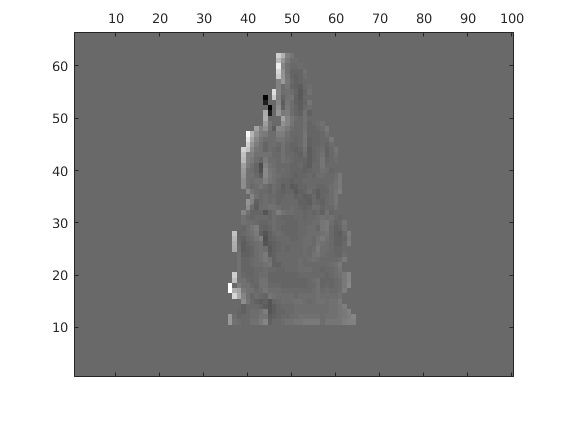
\includegraphics[width=.4\linewidth]{imagenes/buda_small_dephs_789.png}